\myappendix{tracker}{Tracker Cheat Sheet}

\subsection*{Description}

This one-page ``cheat sheet'' will show you the most common steps required to analyze videos with Tracker.Tracker is developed by Doug Brown and is available from \url{http://www.cabrillo.edu/~dbrown/tracker/}.

\subsection*{Preliminary Steps}

\begin{enumerate}
	\item Go to \menu{Video$\to$Import\dots} and select the video you wish to analyze.
	
	\scaledimage{./appendix-tracker/import}{Import your video.}{0.3}
	
	\item Click the movie settings icon 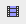
\includegraphics[scale=0.8]{./appendix-tracker/movie-settings} and set the frame rate, start frame, and end frame. Note that setting the start frame and end frame is quite useful for trimming the movie to just the part that is of interest.
	
	\item Click the calibration icon 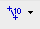
\includegraphics[scale=0.7]{./appendix-tracker/calibration} and select one of the calibration tools. Stretch the tool across an object of known length, such as a meterstick, that is in the plane of the motion. Click on the numeric indicator for the length of the tool and change the value to be the length of your standard object in the video.
	
	\item Click the coordinate system icon 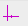
\includegraphics[scale=0.7]{./appendix-tracker/coord-sys} and move the origin of the coordinate system to the desired location. Grab the x-axis and rotate it in order to set the direction of the coordinate system. 	
	
\end{enumerate}

\subsection*{Mark an object}

\begin{enumerate}
	\item Click the \button{Create} button and select \menu{Point Mass}.
	\item In the toolbar, a menu for \menu{mass A} will appear.  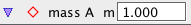
\includegraphics[scale=0.5]{./appendix-tracker/massA} Click on \menu{mass A} in order to select its \menu{Name\dots}, \menu{Color\dots}, or other parameters.
	\item {\bf \emph{While holding the shift key}}, click on the object. A mark will appear, and the video will advance to the next frame.
\end{enumerate}

\subsection*{Analyze a graph}

\begin{enumerate}
	\item Right-click on the graph and select \menu{Analyze\dots}. The Data Tool window will pop up. 
	\item Check \button{\ding{51}}Fit, and the Fit menus and parameters will appear. 
	\item Check \button{\ding{51}}Autofit for the Data Tool to automatically calculate the best-fit parameters.
	\item To fit a curve to a portion of the data, select the data in the graph or data table.
\end{enumerate}
